\begin{frame}
    \frametitle{Konsequenzen der Riemannschen Hypothese}
        %plot with pi(x) and Li(x)
        %\item Cramer: $p_{k+1} - p_k = \mathcal{O}(\sqrt{p_k}\log p_k)$.
        %De la Vallée-Poussin: $\pi(x) - \operatorname{Li}(x) = \mathcal{O}(xe^{-a\sqrt{\log(x)}})$
        \only<1>{
            \begin{figure}
                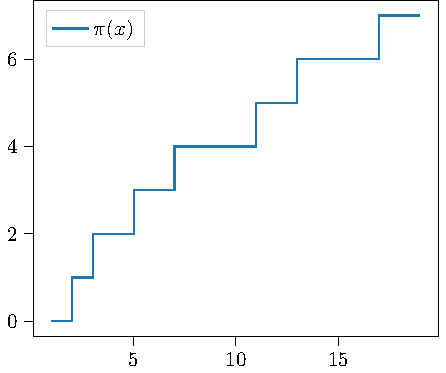
\includegraphics[scale=0.8]{figures/pi_plot.pdf}
                \caption{$\pi(x)$}
            \end{figure}
        }
        \only<2>{
            \begin{figure}
                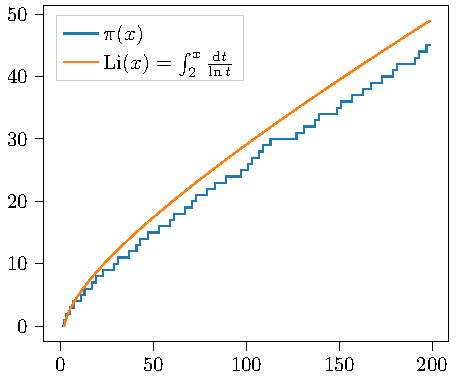
\includegraphics[scale=0.8]{figures/pi2_plot.pdf}
                \caption{Eine Annäherung für $\pi(x)$.}
            \end{figure}
        }
        \only<3>{
            \begin{figure}
                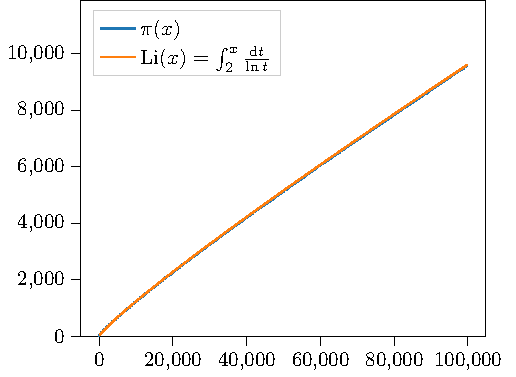
\includegraphics[scale=0.8]{figures/pi_li_none_plot.pdf}
                \caption{Eine Annäherung für $\pi(x)$}
            \end{figure}
        }
        \only<4>{
            \begin{figure}
                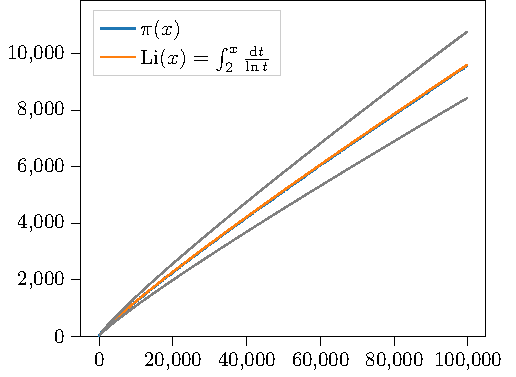
\includegraphics[scale=0.8]{figures/pi_li_trudgian_plot.pdf}
                \caption{$|\pi(x) - \operatorname{Li}(x)| \leq 0.2795{\frac {x}{(\log x)^{3/4}}}\exp \big(-{\sqrt {\frac {\log x}{6.455}}}\big)\forall x \geq 229$}
            \end{figure}
        }
        \only<5>{
        \begin{figure}
            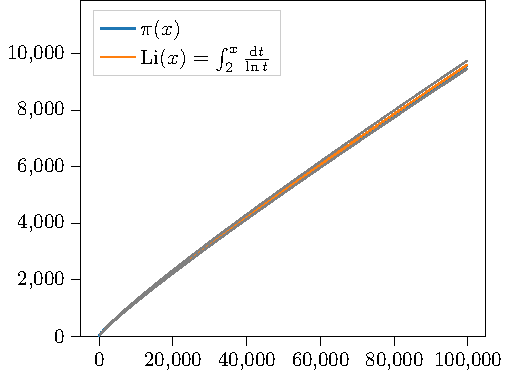
\includegraphics[scale=0.8]{figures/pi_li_rh_plot.pdf}
            \vspace*{-1.5pt}
            \caption{$|\pi(x) - \operatorname{Li}(x)| < \frac{\sqrt{x}\log(x)}{8\pi}\forall x \geq 2657$}
        \end{figure}
        }
\end{frame}